\chapter{Literature Review} \label{chapter:literature_review}
The development of reliable and scalable ASR systems requires an understanding of modern distributed systems technologies and architectural design. This literature review examines the technologies and approaches relevant to enhancing ASR system scalability and resilience. The review begins with an introduction to the key technologies in distributed systems, containerization cloud infrastructure, chaos enginnering and message queues. It then discussed the previous work on the ASR system and explore the research gap.

\section{Distributed Systems Architecture}
\subsection{Evolution of Microservices}
The transition from monolithic to microservices architecture represents a fundamental shift in distributed systems design. Newman \cite{newman} defines microservices as small, autonomous services that work together, focusing on modularity and independent deployability. This architectural style has gained prominence due to its ability to support scalability, maintainability, and team autonomy \cite{microservices_benefits}. In the context of ASR systems, microservices architecture enables independent scaling of components and improved fault isolation.

\subsection{gRPC in Modern Applications}
gRPC is a high-performance Remote Procedure Call (RPC) framework \cite{grpc} that has significantly advanced service-to-service communication. It leverages Protocol Buffers, a language-agnostic interface definition language \cite{protocol_buffers}, enabling seamless communication between services written in different programming languages. This is particularly beneficial in microservices architectures, where different teams may develop services using diverse technology stacks. 

Performance analyses by Niswar et al. \cite{grpc_comparison} demonstrate that gRPC outperforms REST APIs and GraphQL in response time for retrieving both flat and nested data while also exhibiting lower CPU utilization. These advantages make gRPC particularly well-suited for ASR systems, where efficient, low-latency communication between components is crucial.

\subsubsection{gRPC Architecture}

Figure \ref{fig:grpc} illustrates the gRPC architecture, which consists of the following key components:
\begin{enumerate}
    \item \textbf{Client}: The application that initiates gRPC calls.
    \item \textbf{Server}: The application that implements the gRPC service and processes incoming requests.
    \item \textbf{Protocol Buffers}: A language-agnostic schema used to define services and message structures.
    \item \textbf{gRPC Stub}: The auto-generated client and server code derived from Protocol Buffer definitions.
    \item \textbf{Hypertext Transfer Protocol (HTTP)/2}: The transport protocol used to facilitate efficient and multiplexed communication.
\end{enumerate}

\begin{figure}[H]
    \centering
    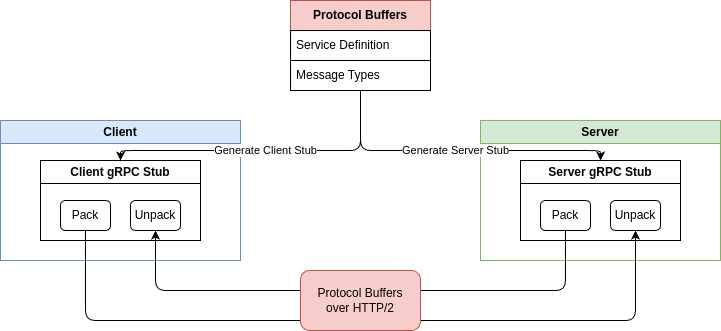
\includegraphics[width=\textwidth]{figures/gRPC_architecture.drawio.png}
    \caption{gRPC Architecture}
    \label{fig:grpc}
\end{figure}

\subsubsection{gRPC Communication Process}
The process begins with defining the service and message types using Protocol Buffers \cite{protocol_buffers_overview}. The \texttt{protoc} compiler then generates the client and server code. The client application uses the generated client stub to make a gRPC call \cite{grpc_api}, sending a request over HTTP/2 \cite{grpc_http2}. The server application uses the generated server stub to handle the gRPC call, processes the request, and sends back a response  over HTTP/2 \cite{grpc_api}.


\section{Containerization}
\subsection{Docker}
Docker is a service that utilizes operating system-level virtualization to package software into lightweight, portable containers \cite{docker_definition}. Each Docker container bundles an application together with its required dependencies, ensuring consistent behavior across different environments \cite{container_definition}. This consistency is particularly vital for ASR systems, where managing complex model dependencies and service configurations is essential for reliable performance.
\subsection{Kubernetes}
Kubernetes is a container orchestration tool used to automate the deployment and management of containers \cite{k8s_definition}. 

A Kubernetes cluster (Figure \ref{fig:kubernetes_architecture}) contains the following key components \cite{k8s_cluster}:
\begin{enumerate}
    \item \textbf{Control Plane}: Consists of the following components:
    \begin{itemize}
        \item \textbf{Application Programming Interface (API) Server}: Exposes the Kubernetes API.
        \item \textbf{etcd}: Key-value store for cluster data.
        \item \textbf{Scheduler}: Assigns workloads to nodes.
        \item \textbf{Controller Manager}: Ensures the desired state of the cluster.
        \item \textbf{Cloud Controller Manager}: Integrates with cloud provider APIs.
    \end{itemize}
    \item \textbf{Worker Nodes}: The compute nodes that run containerized applications.
    \begin{itemize}
        \item \textbf{Kubelet}: Agent that manages the node and communicates with the control plane.
        \item \textbf{Container Runtime}: Software that runs containers.
        \item \textbf{Kube Proxy}: Manages network connectivity.
    \end{itemize}
\end{enumerate}

\begin{figure}[H]
    \centering
    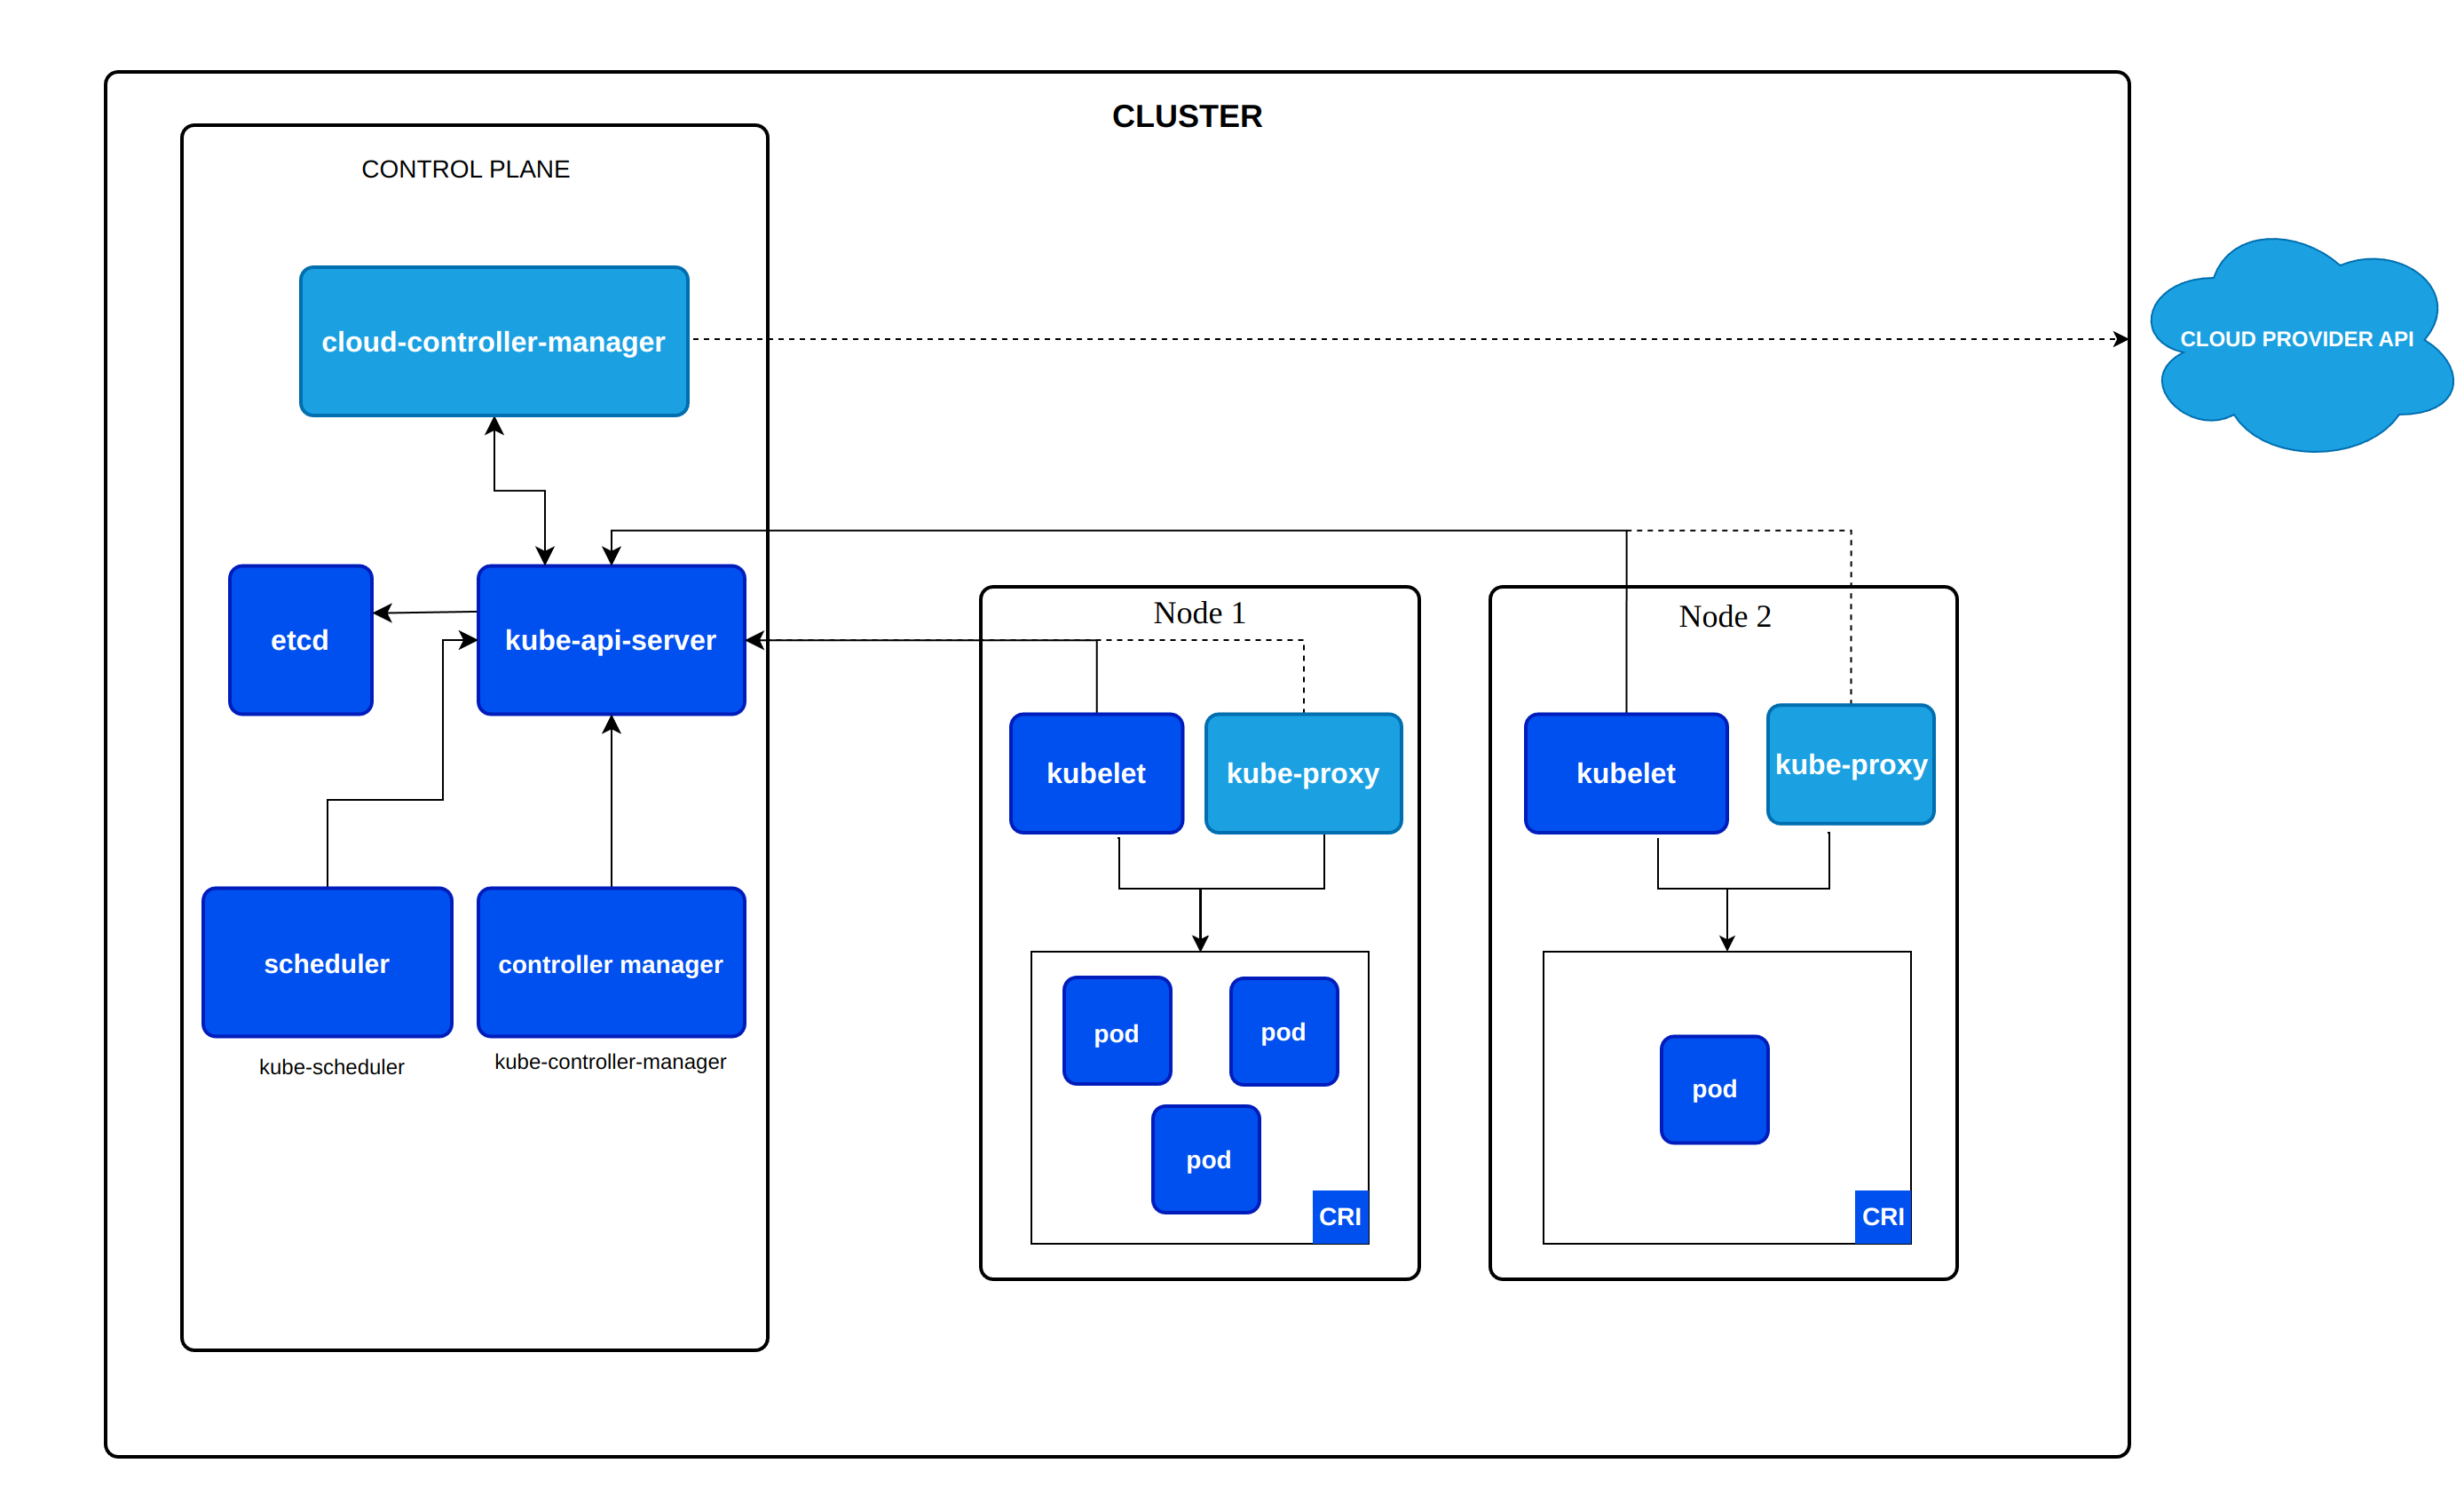
\includegraphics[width=\textwidth]{figures/kubernetes_architecture.png}
    \caption{Kubernetes Cluster Architecture \cite{k8s_cluster}}
    \label{fig:kubernetes_architecture}
\end{figure}

Burns et al. \cite{k8s_architecture} detail its architecture and ability to manage containerized applications at scale. For ASR systems, Kubernetes provides essential features such as automatic scaling, self-healing, and rolling updates \cite{k8s_features}, which are crucial for maintaining service reliability.

\subsection{Helm}
Helm is a package manager for Kubernetes applications \cite{helm_definition}. Helm utilises Charts, as reusable packages that contains pre-configured Kubernetes resources \cite{helm_charts}, making complex application deployments more manageable. These Charts function as templates that can be customized through value files \cite{helm_definition}, enabling environment-specific configurations while maintaining consistency in the underlying architecture.

\section{Amazon Web Services (AWS)}
AWS is a cloud service provider that offers a wide range of products and services. These services span compute, storage, networking, database, and container management, among others \cite{aws_definition}.

\subsection{Virtual Private Cloud (VPC)}
Amazon VPC forms the networking foundation for AWS resources, providing an isolated virtual network environment in the cloud \cite{vpc}. It enables users to define network architecture with custom IP address ranges, subnets, and routing tables \cite{vpc}. A key feature is its ability to span multiple Availability Zones (AZs) within a region, enhancing system resilience through geographical distribution \cite{vpc_az}.

\subsection{Elastic Compute Cloud (EC2)}
Amazon EC2 is a computing service that provides scalable virtual machines (instances) in the cloud \cite{ec2_definition}. It offers a wide range of instance types optimized for different use cases, from compute-intensive applications to memory-intensive workloads \cite{ec2_instance_types}. EC2 instances can be launched across multiple AZs for high availability. EC2 pricing models including on-demand, reserved, and spot instances to optimize costs based on workload patterns \cite{ec2_pricing}.

\subsection{Identity and Access Management (IAM)}
IAM provides fine-grained access control to AWS resources \cite{iam_definition}. It implements the principle of least privilege through a comprehensive policy framework that defines who (principal) can do what (actions) on which resources under specific conditions \cite{iam_security}. IAM enables organizations to manage user identities, roles, and permissions centrally, ensuring secure access to cloud resources while maintaining compliance requirements.

\subsection{Elastic Kubernetes Service (EKS)}
Amazon EKS is a managed Kubernetes service that simplifies the deployment, management, and scaling of containerized applications \cite{eks_definition}. It automatically manages the availability and scalability of the Kubernetes control plane across multiple AZs \cite{eks_definition}. EKS integrates seamlessly with other AWS services and supports various deployment models, including hybrid architectures that span cloud and on-premises environments \cite{eks_deployment}.

\subsection{Elastic Container Registry (ECR)}
Amazon ECR is a managed container registry service that simplifies the storage, management, and deployment of container images \cite{ecr_definition}. It provides encrypted image storage and integrates with AWS IAM for access control \cite{ecr_iam}. ECR features automatic image scanning for vulnerabilities \cite{ecr_image_scanning} and lifecycle policies for image management \cite{ecr_lifecycle}, making it an essential component in container-based architectures.

\subsection{Elastic File System (EFS)}
Amazon EFS provides scalable, fully managed network file storage for use with AWS cloud services and on-premises resources \cite{efs_definition}. Supporting the Network File System version 4 (NFSv4) protocol \cite{efs_work}, EFS can be accessed concurrently by thousands of compute instances \cite{efs_performance}. It automatically scales throughput when files are added or removed \cite{efs_performance}, making it ideal for applications requiring shared file access across multiple instances or containers.

\subsection{Elastic Block Store (EBS)}
Amazon EBS is a block storage service that is highly performant and scalable \cite{ebs_definition}. It can be used with EC2 instances to provide persistent storage volumes for EKS \cite{ebs_with_eks}. EBS volumes support various types, including General Purpose SSD (gp2), Provisioned IOPS SSD (io1), and Throughput Optimized HDD (st1) \cite{ebs_types}, enabling users to select the appropriate storage type based on performance requirements.

\section{Infrastructure-as-Code (IaC)}
IaC is an approach to managing and provisioning computing infrastructure through  configuration files, rather than through physical hardware configuration or interactive configuration tools. This method allows for the automation of infrastructure setup, ensuring consistency and reducing the risk of human error \cite{iac_benefits}.

\subsection{Terraform}
Terraform is an IaC tool that allows for the declarative management of cloud resources \cite{terraform_hashicorp}. This means that we define the desired final state of our architecture, and Terraform will apply changes only when necessary to achieve that state \cite{terraform_declarative}. Unlike traditional manual deployment through cloud provider consoles (often referred to as "ClickOps" \cite{clickops}), Terraform enables organizations to define their infrastructure using declarative configuration files. This code-driven approach transforms infrastructure deployment from a manual, error-prone process into an automated, version-controlled workflow.

Terraform enables teams to consistently replicate environments across development, testing, and production stages \cite{iac_benefits}, ensuring that infrastructure configurations remain identical at each phase. By maintaining infrastructure as code, teams can version control their changes, enabling peer reviews and the ability to roll back modifications if issues arise. Terraform also manages dependencies between different cloud resources automatically \cite{terraform_dependencies}, reducing the complexity of infrastructure deployment. 

\section{Chaos Engineering}
Chaos engineering is a proactive approach to identifying system weaknesses by deliberately introducing failures \cite{chaos_engineering_definition}. By simulating conditions like Kubernetes pod failure, network delay, and node stress \cite{chaos_mesh_feature}, chaos engineering helps us observe system behaviour under stress and improve system robustness \cite{chaos_engineering_definition}. It also enhances incident response time by enabling a better understanding of failure scenarios \cite{chaos_engineering_definition}. Some chaos engineering tools include Chaos Mesh \cite{chaos_mesh_introduction} and AWS Fault Injection Simulator (FIS) \cite{fis_introduction}.\enlargethispage{1\baselineskip}

\section{In-memory Data Storage}
\subsection{Redis}
Redis is a high-performance, in-memory data store commonly used as a cache and a key-value database \cite{redis_definition}. Redis is fast, and thus well-suited for use in ASR systems, where it can store session information and temporary transcription data. This enables rapid access to frequently used data and facilitates reliable state management, ensuring smooth and responsive system performance. 

To achieve high availability, Redis can be configured with replication to keep it in sync with the primary instance \cite{redis_replication}. Redis Sentinel can be used to monitor Redis instances and perform automatic failover in case of primary instance failure \cite{redis_sentinel}. A group of Redis instances can be configured to be in sentinel mode, which can detect the failure of the primary Redis instance through a quorum and promote a replica to the primary (Figure \ref{fig:redis_sentinel}).

\begin{figure}[H]
    \centering
    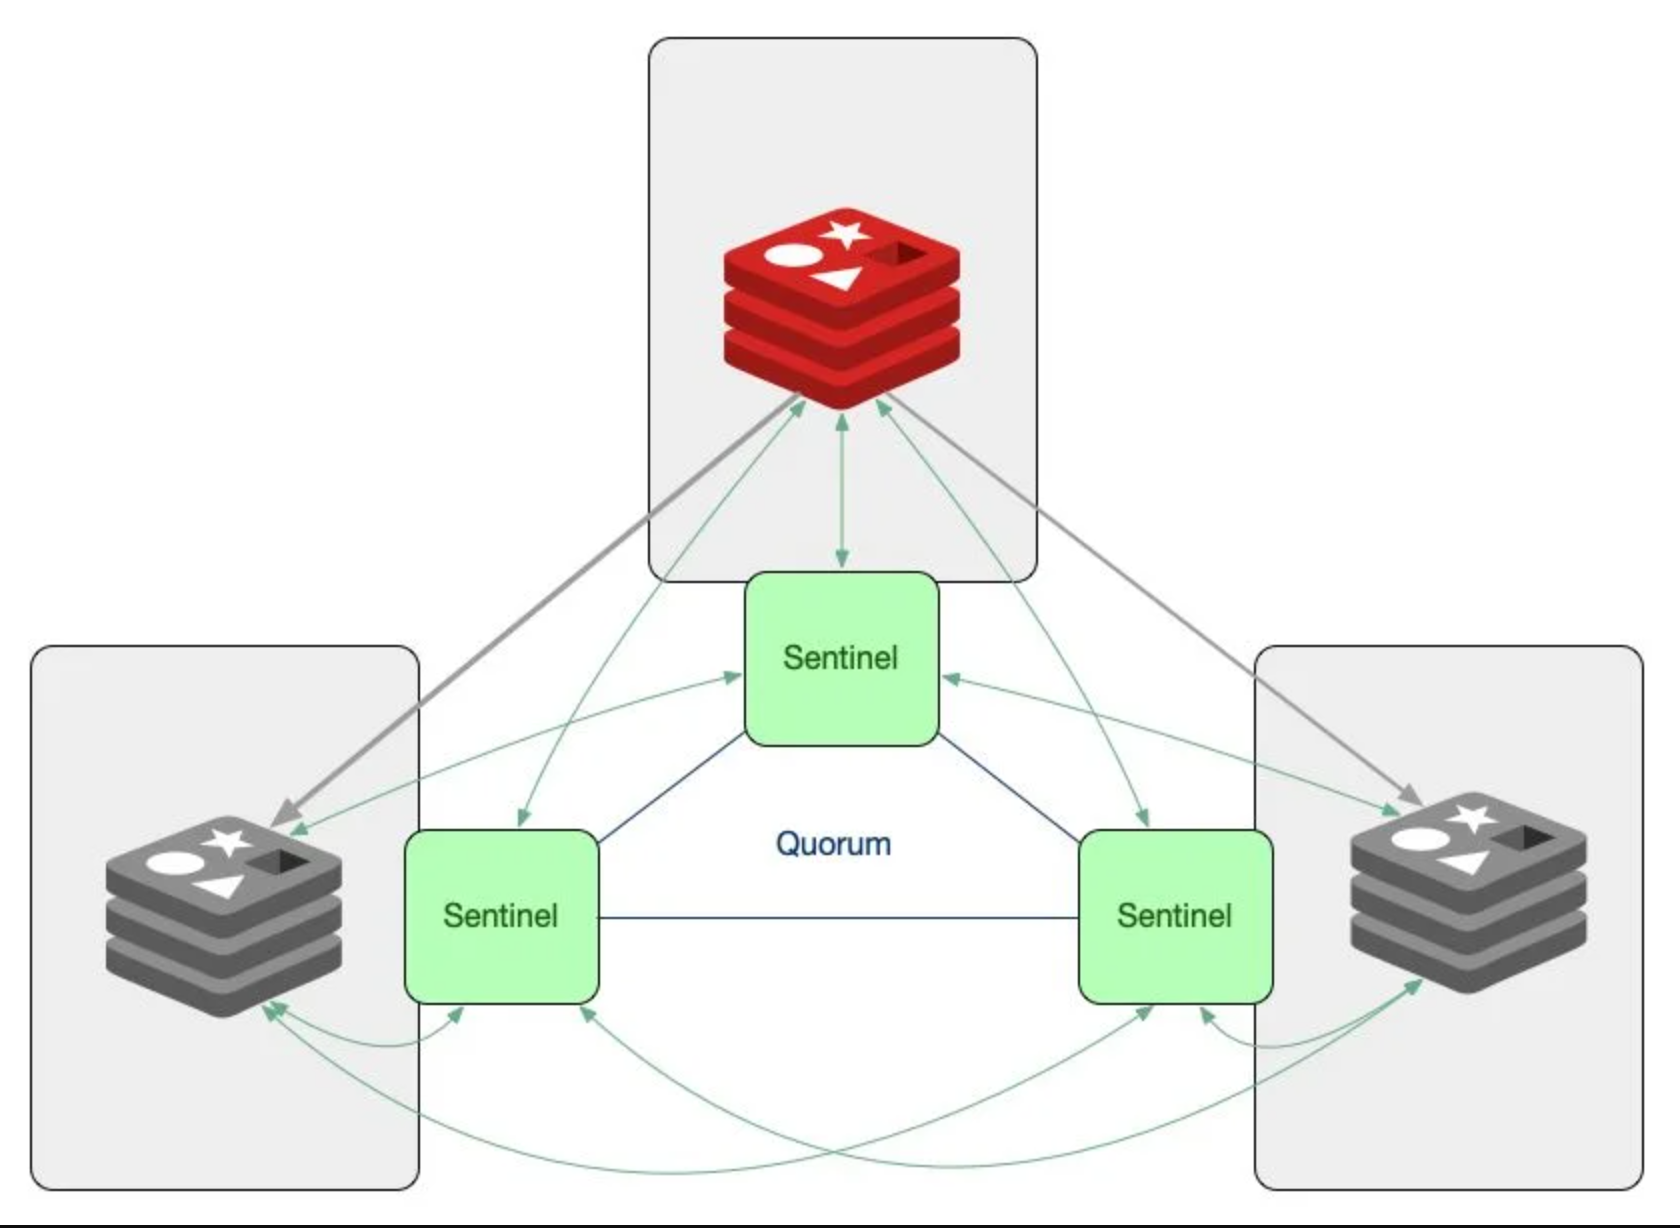
\includegraphics[width=0.8\textwidth]{figures/redis_sentinel.png}
    \caption{Redis Sentinel}
    \label{fig:redis_sentinel}
\end{figure}

\section{Message Queues}
Message queues enable asynchronous communication between services in distributed systems, providing temporary message storage and reliable delivery mechanisms \cite{queue_definition}. This asynchronous pattern facilitates decoupling of producers and consumers \cite{queue_decouple}, allowing components to scale independently and operate without direct dependencies on each other. This section compares Apache Kafka and RabbitMQ, two popular message brokers, to determine the most suitable choice for ASR systems.
\subsection{Apache Kafka}
Apache Kafka is designed as a distributed log-based messaging system, and its main use case is for ingesting and streaming real-time data \cite{kafka_definition}. Kafka's architecture centers around append-only logs (topics) divided into partitions, where messages are immutably stored and accessed via offset-based positioning \cite{kafka_documentation}.

Figure \ref{fig:kafka_partitioning} illustrates Kafka's partitioning mechanism, where messages are distributed across partitions within a topic.This partitioning enables Kafka to achieve high throughput by allowing multiple consumers to read messages concurrently from different partitions \cite{kafka_parallel}.
\begin{figure}[H]
    \centering
    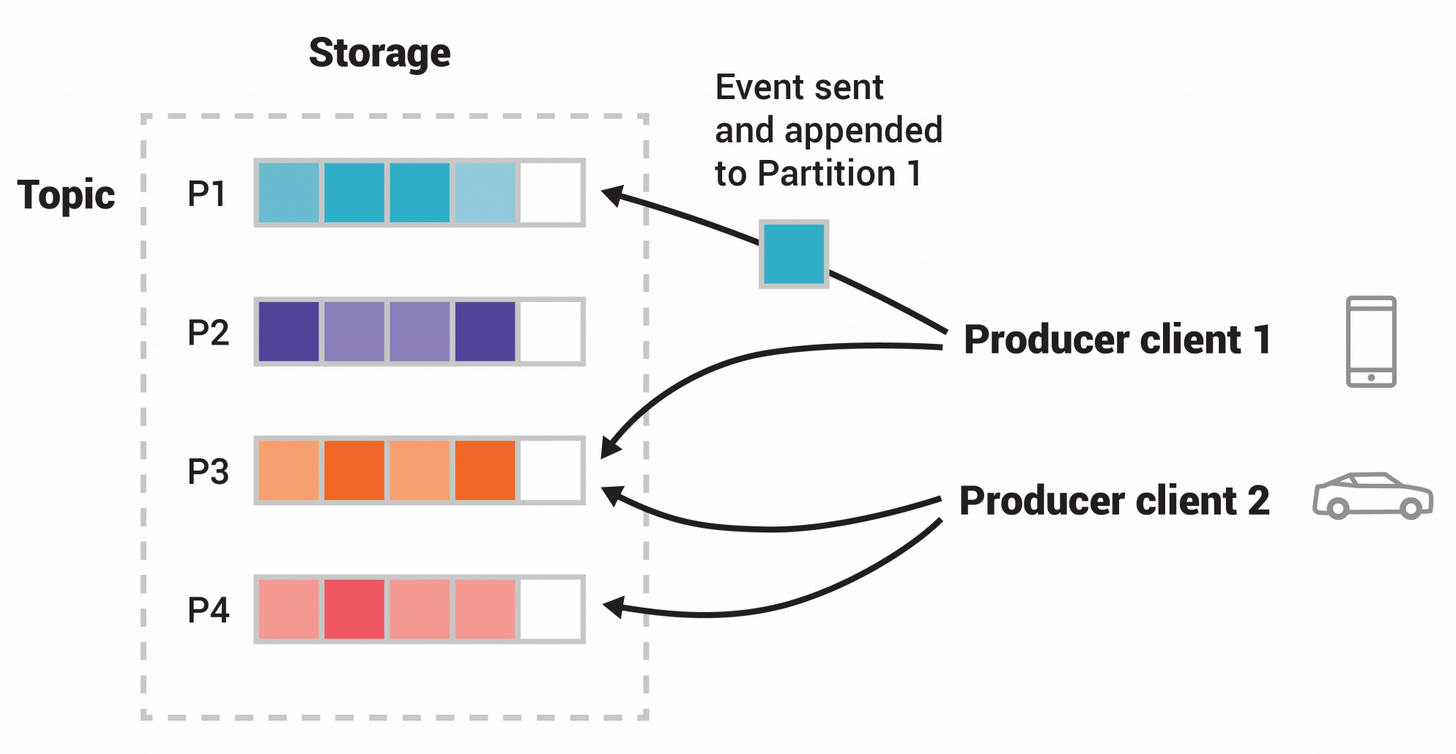
\includegraphics[width=\textwidth]{figures/kafka_topics_partition.png}
    \caption{Kafka Topic Partitioning \cite{kafka_partitions}} 
    \label{fig:kafka_partitioning}
\end{figure}

\subsection{RabbitMQ}
RabbitMQ implements the Advanced Message Queuing Protocol (AMQP) \cite{rabbitmq_protocols} and operates as a broker-based message queue \cite{rabbitmq_definition}. It provides sophisticated message routing capabilities through exchanges and queues, supporting various patterns including publish-subscribe, and request-reply communications \cite{rabbitmq_routing}. RabbitMQ offers features such as message acknowledgments, dead letter queues, and priority queuing \cite{rabbitmq_routing}, making it particularly suitable for complex message routing requirements.

In RabbitMQ, producers send messages to exchanges, which then route them to queues based on predefined routing rules \cite{rabbitmq_routing}. Consumers subscribe to queues to receive messages, while RabbitMQ ensures reliable message delivery through message acknowledgments \cite{rabbitmq_ack}. 

Figure \ref{fig:rabbitmq_routing} illustrates RabbitMQ's message routing process through different exchanges. 

\begin{figure}[H]
    \centering
    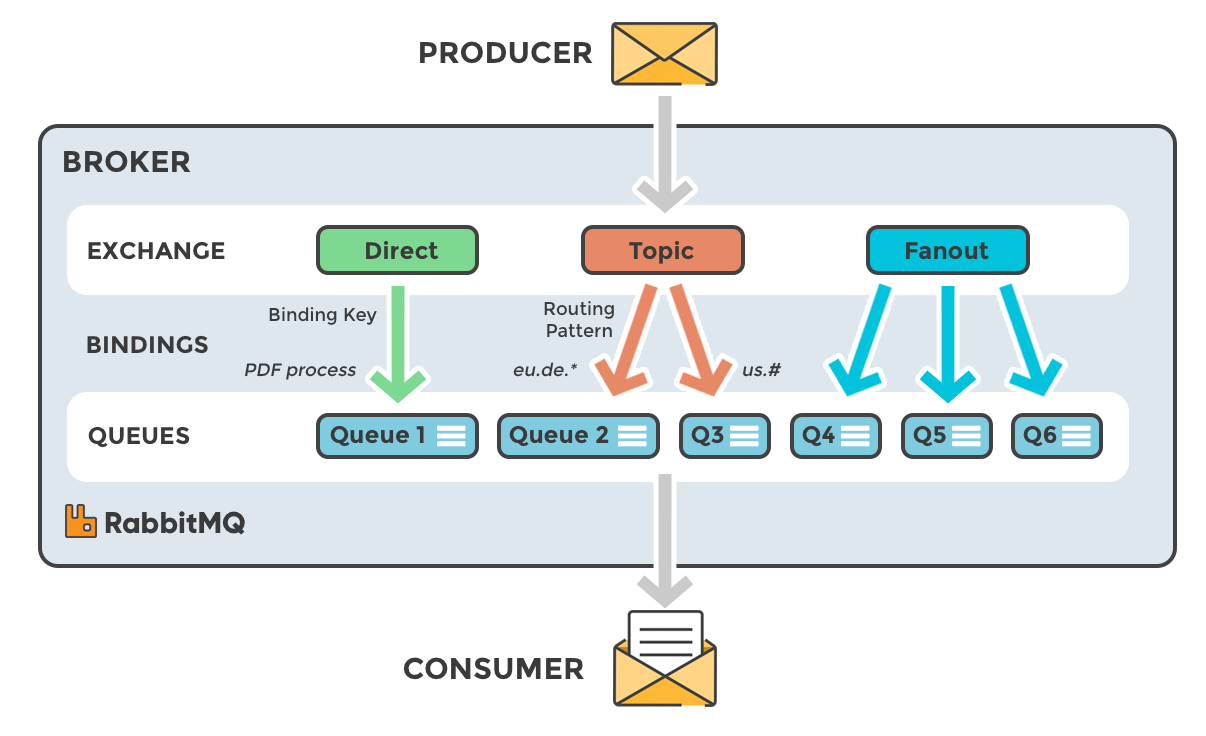
\includegraphics[width=\textwidth]{figures/exchanges-topic-fanout-direct.png}
    \caption{RabbitMQ Message Routing \cite{rabbitmq_diagram}}
    \label{fig:rabbitmq_routing}
\end{figure}

There are four main types of exchanges in RabbitMQ \cite{rabbitmq_exchanges}:
\begin{enumerate}
    \item \textbf{Direct Exchange}: Routes messages to queues based on the binding key.
    \item \textbf{Fanout Exchange}: Routes messages to every queue bound to the exchange.
    \item \textbf{Topic Exchange}: Routes messages based on routing patterns.
    \item \textbf{Default Exchange}: Routes messages to queues based on the queue name.
\end{enumerate}

\subsection{Comparison of Kafka and RabbitMQ}
While both systems are robust message brokers, their architectural differences significantly impact their suitability for ASR applications. This section compares them across key dimensions relevant to ASR systems.

\subsubsection{Message Ordering}
Kafka's partitioned architecture, while enabling high throughput, cannot guarantee message ordering across partitions. As noted by Dobbelaere and Esmaili \cite{kafka_v_rabbitmq}, Kafka's ordering guarantees are confined to individual partitions only.

In contrast, RabbitMQ employs a queue-based architecture that enforces strict First-In-First-Out (FIFO) ordering within each queue and channel \cite{kafka_v_rabbitmq}. This characteristic makes RabbitMQ more suitable for live transcription ASR systems, where preserving the sequence and context of speech data is essential for accurate transcription.

\subsubsection{Message Delivery Guarantees} Kafka ensures at-least-once delivery semantics through offset management \cite{kafka_v_rabbitmq}. However, consumers must carefully manage offset commits to prevent reprocessing or potential data loss.

RabbitMQ, on the other hand, offers more flexible delivery guarantees via its acknowledgment mechanism \cite{kafka_v_rabbitmq}. It supports both positive acknowledgments and negative acknowledgments (NACKs), allowing unprocessed messages to be requeued automatically \cite{rabbitmq_nack}. These features are advantageous for ASR systems, where reliability, data integrity, and the prevention of audio data loss are crucial.

\subsubsection{Processing Requirements}
For ASR systems, where maintaining speech context is paramount \cite{speech_context}, RabbitMQ's single-queue consumer model aligns better with the need for sequential processing for live transcription tasks.

While Kafka provides a throughput advantage for high-volume streaming \cite{kafka_v_rabbitmq}, its partitioned structure does not guarantee sequential audio data processing, as speech context cannot be split across partitions. Since live transcription requires sequential audio processing, RabbitMQ is the more suitable choice for this use case.

\subsubsection{Message Queue Selection} \label{subsection:research_gap}
Based on these considerations and supported by Dobbelaere and Esmaili's \cite{kafka_v_rabbitmq} findings, RabbitMQ emerges as the more appropriate choice for ASR systems due to its strong message ordering guarantees, flexible acknowledgement mechanisms, and support for sequential processing requirements. By leveraging RabbitMQ's features, ASR systems can ensure accurate transcription results and maintain the context of speech data for live transcription throughout the processing pipeline.


\section{Previous Work}
Putra \cite{putra} had worked on the same ASR system and his project effectively highlights the advantages of transitioning from a tightly coupled ASR system to a decoupled microservices architecture using Apache Kafka. The use of Kubernetes and other modern cloud-native tools such as Kyverno, Falco, and Knative demonstrates a robust effort to address scalability, reliability, and security challenges in ASR systems. The project discusses the integration of Kafka as the message broker to decouple the master and worker components, ensuring fault tolerance and enabling the system to recover from worker crashes without losing data.

\subsection{Research Gap}
A critical research gap exists in the selection of message broker technology for ASR systems. The selection of Kafka for the ASR system raises concerns regarding its fit for scenarios requiring high data accuracy and context preservation. ASR systems are inherently constrained by the processing speed of workers rather than the message broker, making Kafka’s high throughput less impactful. Additionally, due to the sequential nature of speech processing, audio data cannot be effectively partitioned across multiple Kafka partitions. As a result, the system fails to leverage Kafka’s parallel processing advantages, leading to an architectural misalignment between technology choice and system requirements.

In contrast, RabbitMQ provides robust acknowledgment and message ordering guarantees, making it better suited for ASR tasks that require strict message sequencing and sequential processing. Consequently, RabbitMQ may offer a more suitable alternative for ensuring accurate and context-aware transcription.

Furthermore, while Putra’s work \cite{putra} demonstrated promising results, a practical limitation emerged as the research team no longer has access to his project's codebase. This circumstance has created an opportunity to revisit the system's architecture with fresh perspective, particularly in the areas of component decoupling and scaling mechanisms. The current project therefore aims to not only address the technological fit of the message broker but also to establish a well-documented implementation that can be maintained and evolved by the research team.

